%
\section{Introduction}%
%
\begin{frame}%
\frametitle{Quick Overview}%
\begin{itemize}%
\item Concept of optimization algorithms% 
\item<2-> How to benchmark such algorithms%
\item<3-> How to evaluate data obtained from benchmarking and how to compare algorithms
\item<4-> The \optimizationBenchmarking\ Framework can do it for you!%
\item<7-> It provides a graphical user interface in a client/server application for loading, editing, and evaluating experimental results.%
\item<8-> It can run as Docker container under Linux, MacOS?, and Windows? without needed any additional software (except Docker and a browser).% 
\item<9-> It produces reports, similar to articles, in \LaTeX\ with figures and building blocks ready for use in your publications%
\end{itemize}%
\end{frame}%
%
%
\begin{frame}[t]%
\frametitle{Optimization}%
\begin{itemize}%
\item Many questions in the real world are actually optimization problems\only<2->{, e.g.,\only<-8>{%
\begin{itemize}%
%
\item \only<-5>{Find the \emph{shortest} tour for a salesman to visit certain set of cities\only<-2>{ in China and return to Hefei!}}\only<6->{\alert<6>{Traveling Salesman Problem}\scitep{ABCC2006TTSPACS,LLKS1985TTSPAGTOCO,GP2004TTSPAIV,L2011SGEFTSPIMSS}}%
%
\item<3-> \only<-5>{I need to transport $n$ items from here to another city\only<-3>{ but they are too big to transport them all at once. How can I load them best into my car so that I have to travel back and forth the least times?}}\only<6->{\alert<6>{Bin Packing Problem}\scitep{KSH1995EHFTBPP}}%
%
\item<4-> \only<-5>{Which setting of $x_1$, $x_2$, $x_3$, and $x_4$ can make $(x_1\lor\lnot x_2 \lor x_3)\land(\lnot x_2\lor\lnot x_3 \lor x_4) \land (\lnot x_1\lor\lnot x_3 \lor \lnot x_4)$ become true\only<-4>{ (or, at least, as \emph{many} of its terms as possible)?}}\only<6->{\alert<6>{Maximum (3-)Satisfiability Problem}\scitep{HS2000SAORFROS,TH2004UAIAEEFSAFSAMS,S1978TCOSP,RMK2000EASP}}%
%
\item<5-> \only<-5>{I want to build a large factory with $n$ workshops. I know the flow of material between each two workshops and now need to choose the locations of the workshops such that the overall running cost incurred by material transportation is \emph{minimized}.}\only<6->{\alert<6>{Quadratic Assignment Problem}\scitep{MF1999ACOMATSAACFTQAP,GTD1999ACOQAP}}%
\end{itemize}%
}\only<9->{ the Traveling Salesman Problem\scitep{ABCC2006TTSPACS,LLKS1985TTSPAGTOCO,GP2004TTSPAIV,L2011SGEFTSPIMSS}}%
}%
%
\item<7-> Many optimization problems are \alert<7>{\NPHard}, meaning that finding the best possible solution will usually not be possible in \alert<8>{feasible time}.%
%
\item<11-> It is easy to get \emph{some} solutions (usually of bad quality)%
%
\item<12-> We use metaheuristic optimization algorithms to give us good approximate solutions within acceptable runtime.%
\item<13-> Examples of such algorithms are\only<-23>{ %
Evolutionary Algorithms\scitep{BFM1997EA,CWM2011VOEAFRWA,BFM2000EC1BAAO,BFM2000EC2BAAO,DLJD2000EC,EM1999EC,CDGDMPP1999NIIO,GT2002AIECTAA,WGOEB}\uncover<14->{, %
Ant Colony Optimization\scitep{DMC1996ACO,DS2004ACO,GM2002APBATDOP,ZBMD2004MBSFCOACS,WGOEB}\uncover<15->{, %
Evolution Strategies\scitep{R1965ES,R1973ES,R1994ES,S1965KYASDEFIDS,S1968EOEZDT1,S1975EUNO,WGOEB}\uncover<16->{, %
Differential Evolution\scitep{PSL2005DE,F2006DE,WGOEB}\uncover<17->{, %
Particle Swarm Optimization\scitep{KE1995PSO,C2006PSO,WGOEB}\uncover<18->{, %
Estimation of Distribution Algorithms\scitep{PSL2005DE,F2006DE,MMVRCC2006DE,BZSM2006DE,LZ2000DE,MM2005DE,BVPK2006DE,S2010DEFCFOAABKPARS}\uncover<19->{, %
CMA-ES\scitep{HOG1995ESAD,HO1996AANMDIESTCMA,HO2001ESCMA,HMK2003RTTCOTDESWCMACE,HK2004ETCESOMTF,H2006TCESACR,AH2005ARCESWIPS,AH2005PEOAALSEA}\uncover<20->{, and %
Local Search methods\scitep{HS2005SLSFAA,AL1997LSICO,DBSD2001DOILSA}\uncover<21->{ such as %
Simulated Annealing\scitep{SSF2002FCAIFSA,LA1987SATAA,B1987GAASA,JCS2003HC,KGV1983SA,VC1985SA,DPSW1982MCTICO,DPSW1982MCTICO2,P1970AMCMFTASOCTOCOP,WGOEB}\uncover<22->{ or %
Tabu Search\scitep{G1989TSPI,G1990TSPII,GL1993TABU,DWH1989TSTATAAATNN,BT1994TABU}\uncover<23->{, %
as well as hybrids of local and global search, such as Memetic Algorithms\scitep{M1989MA,M2002MA,MC2003AGITMA,ES2003HWOTMA,HKS2005RAIMA,DM2004MA,RS1994FMA}%
}}}}}}}}}}}\only<24->{\dots\ many}%
%
\item<24-> \alert<24>{Which of them is best (for my problem)?}%
\item<25-> \alert<25>{How can I make a good algorithm better (for my problem)?}%
%
\end{itemize}%
%
\locateGraphic{2}{width=0.6\paperwidth}{graphics/problem_examples/tsp/tsp}{0.2}{0.29}%
\locateGraphic{3}{width=0.875\paperwidth}{graphics/problem_examples/bin_packing/bin_packing}{0.0625}{0.495}%
\locateGraphic{4}{width=0.55\paperwidth}{graphics/problem_examples/sat/sat}{0.225}{0.5}%
\locateGraphic{5}{width=0.85\paperwidth}{graphics/problem_examples/qap/qap}{0.075}{0.625}%
\locateGraphic{7-8}{width=0.65\paperwidth}{graphics/exponential_functions/exponential_functions}{0.175}{0.6}%
%
\locateGraphic{9}{width=0.75\paperwidth}{graphics/optimization_concept/optimization_concept_1}{0.125}{0.54}%
\locateGraphic{10}{width=0.75\paperwidth}{graphics/optimization_concept/optimization_concept_2}{0.125}{0.54}%
\locateGraphic{11}{width=0.75\paperwidth}{graphics/optimization_concept/optimization_concept_3}{0.125}{0.54}%
\locateGraphic{12}{width=0.75\paperwidth}{graphics/optimization_concept/optimization_concept}{0.125}{0.54}%
%
\end{frame}%
%
%
\begin{frame}[t]%
\frametitle{Algorithm Analysis and Comparison}%
\begin{itemize}%
\item \alert{Which of the algorithms is best (for my problem)?}%
\item<2-> Traditional Approach: Complexity Analysis, Theoretical Bounds of Runtime and Solution Quality%
\item<3-> \alert<-9>{Usually not feasible}\uncover<4->{%
\begin{itemize}%
\item analysis extremely complicated\uncover<5->{ since%
\item<5-> algorithms are usually randomized\uncover<6->{ and%
\item<6-> have many parameters (e.g., crossover rate, population size)\uncover<7->{ and%
\item<7-> \inQuotes{sub-algorithms} (e.g., crossover operator, mutation operator, selection algorithm)%
\item<8-> optimization problems also differ in many aspects%
\item<9-> theoretical results only available for toy problems and extremely simplified algorithms\scitep{WWCTL2016GVLSTIOPSOEAP}.%
}}}%
\end{itemize}%
}%
%
\item<10-> \alert{Experimental analysis and comparison only practical alternative.}%
%
\end{itemize}%
\end{frame}%
%
%
%
\begin{frame}%
\frametitle{Performance and Anytime Algorithms}%
%
\emph{\inQuotes{We use metaheuristic optimization algorithms to give us \alert<3->{good approximate solutions} within \alert<4->{acceptable runtime}.}}%
%
\uncover<2->{%
\begin{itemize}%
\item Algorithm performance has two dimensions\scitep{NAFR2010RPBBOB2ES,WCTLTCMY2014BOAAOSFFTTSP}:\uncover<3->{ solution quality\uncover<4->{ and required runtime}}%
\item<5-> Anytime Algorithms\scitep{BD1989STDPP2} are optimization methods which maintain an approximate solution at \emph{any time} during their run and iteratively improve this guess.%
\item<6-> All metaheuristics are Anytime Algorithms.%
\item<7-> Several exact methods like Branch-and-Bound\scitep{LMSK1963AAFTTSP,Z1993TBABACSOTATSP,Z1999TAADFBABACSOTATSP} are Anytime Algorithms.%
\item<8-> Consequence: Most optimization algorithms produce approximate solutions of different qualities at different points during their process.%
\item<9-> Experiments must capture solution quality and runtime data.%
\end{itemize}%
}%
%
\locateGraphic{3}{width=0.55\paperwidth}{graphics/performance/performance_dimensions/performance_dimensions_1}{0.225}{0.542}%
\locateGraphic{4}{width=0.55\paperwidth}{graphics/performance/performance_dimensions/performance_dimensions_2}{0.225}{0.542}%
\locateGraphic{5}{width=0.55\paperwidth}{graphics/performance/performance_dimensions/performance_dimensions}{0.225}{0.542}%
%
\end{frame}%
%
\begin{frame}[t]%
\frametitle{Experimental Procedure}%
\begin{itemize}%
\item In optimization or Machine Learning, the following experimental procedure is often used\uncover<2->{%
\begin{enumerate}%
\item Select a \only<3->{\alert<3>{set of }}benchmark instance\only<3->{\alert<3>{s}}\only<3-7>{:%
\begin{itemize}%
\item multiple instances%
\item<4-> which cover some different problem features%
\item<5-> should be well-known to make results comparable%
\only<-6>{%
\item<6-> e.g., TSPLib\scitep{R1991ATSPL,R1995T9,DACO1995TSPLIB} for the TSP has instances with different numbers of cities and geometries%
}%
\only<-7>{%
\item<7-> e.g., BBOB\scitep{HAFR2012RPBBOBES,NAFR2010RPBBOB2ES,HAFR2009RPBBOB2ES,FHRA2013RPBBOB2POTNF} offers different benchmark functions for numerical optimization problems%
}%
\end{itemize}%
}%
\item<8-> Do experiment\only<12->{\alert<12-13>{s}}\only<9-13>{:%
\begin{itemize}%
\item conduct several independent runs of algorithm for each benchmark instance%
\item<10-> collect algorithm progress information, e.g., as \emph{\inQuotes{runtime bestObjectiveValue}} tuples%
\item<11-> one log file per run, each log file has several such tuples%
\item<12-> repeat for different algorithm parameter settings (e.g., different population sizes of an EA)%
\item<13-> repeat with other algorithms for comparison purposes%
\end{itemize}%
}%
\item<14-> Evaluate the gathered data\only<15->{:\alert<22>{%
\begin{itemize}%
\item draw diagrams of progress of solution quality over time%
\item<16-> draw diagrams of advanced statistical parameters such as ECDF\scitep{HAFR2012RPBBOBES,HS1998ELVAPAR,TH2004UAIAEEFSAFSAMS,WCTLTCMY2014BOAAOSFFTTSP}\only<17->{ and ERT\scitep{HAFR2012RPBBOBES,WCTLTCMY2014BOAAOSFFTTSP}} (over time)%
\item<18-> use statistical tests to compare results (at different points during the runs)%
\item<19-> analyze the impact of benchmark features and algorithm parameters on the above%
\end{itemize}%
}}%
%
\item<20-> Draw conclusions about algorithm performance and parameter settings%
\item<21-> But this is all \emph{very} cumbersome, involves much work and much data\dots%
\end{enumerate}%
}%
\item<22-> \alert{The \optimizationBenchmarking\ framework can automatize much of the evaluation procedure}%
\end{itemize}%
%
\locateWithCaption{6}{%
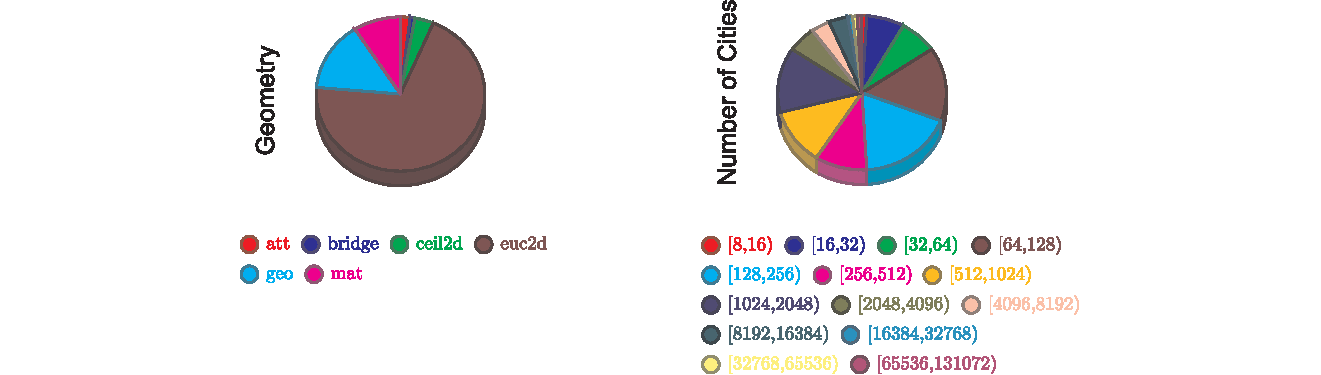
\includegraphics[width=0.925\paperwidth]{graphics/tspLib_features/tspLib_features_symmetric}%
}{%
The relative amounts of the instances of the 110 symmetric instances of TSPLib according to their features (the 10 asymmetric instances are not plotted).%
}{0.0375}{0.51}{0.925}%
%
\locateWithCaption{7}{%
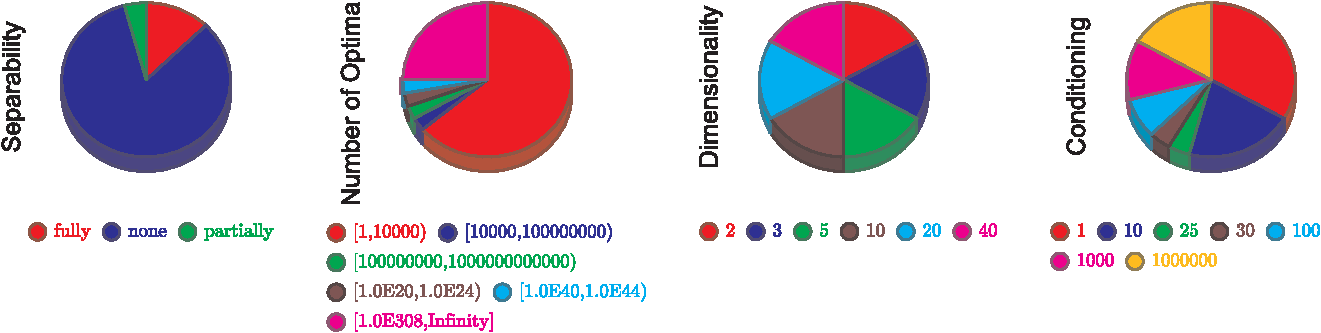
\includegraphics[width=0.925\paperwidth]{graphics/bbob_features/bbob_features}%
}{%
The relative amounts of BBOB benchmark functions according to their features.%
}{0.0375}{0.51}{0.925}%
%
\locateWithCaption{10}{%
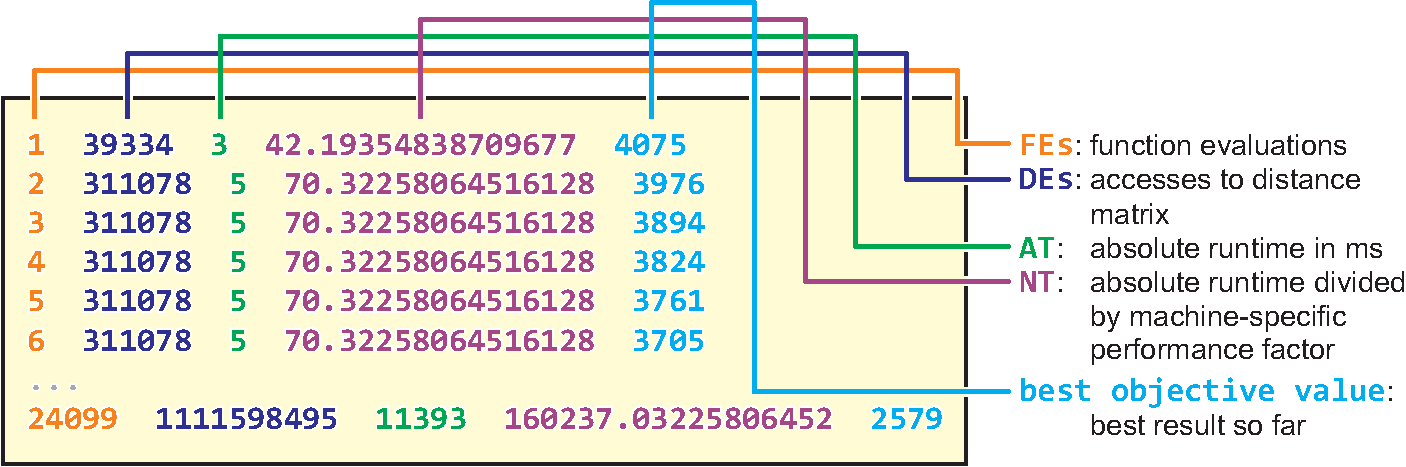
\includegraphics[width=0.8\paperwidth]{graphics/tspSuite_logfile_example/tspSuite_logfile_example}%
}{%
Example for data collected in a log file by TSP~Suite\scitep{WCTLTCMY2014BOAAOSFFTTSP,JWLCA2014CAHBABAWECMLSATHOTT}.%
}{0.0375}{0.53}{0.925}%
%
\locateWithCaption{15-17}{
\strut%
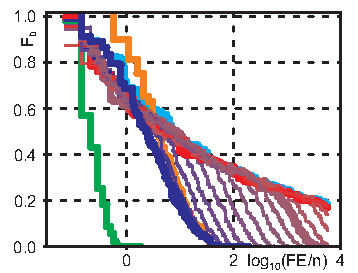
\includegraphics[width=0.28\paperwidth]{graphics/performance/progress_example/progress_example}%
\uncover<16->{%
\strut\hfill\strut%
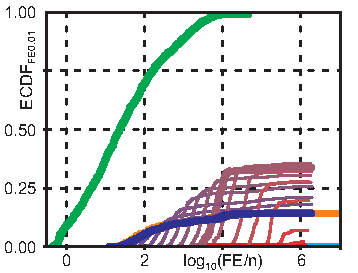
\includegraphics[width=0.28\paperwidth]{graphics/performance/ecdf_example/ecdf_example}%
\uncover<17->{%
\strut\hfill\strut%
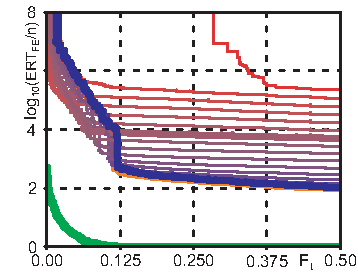
\includegraphics[width=0.28\paperwidth]{graphics/performance/ert_example/ert_example}%
}}\strut%
}{%
Examples for progress\only<16>{ and ERT}\only<17->{, ERT, and ECDF} diagrams for different algorithms (signified by different colors) over different sub-sets of the TSPLib data.%
}{0.0375}{0.525}{0.925}%
%
\end{frame}%

